\documentclass{lzureport}

\usepackage{caption}
\usepackage[dvipsnames]{xcolor}  % 更全的色系
\usepackage{listings}  % 排代码用的宏包
\usepackage{adjustbox}

\usepackage{booktabs}
\usepackage{float}
\usepackage{amsmath}
\usepackage{titlesec}
\usepackage{tabularx,array,makecell}
%\usepackage{color,xcolor}
%\usepackage{cases}
%\usepackage{mathtools}
%\usepackage{tcolorbox}
%\usepackage{tikz}

%%%%%%%%%%%%%%%%%%%%%%%%%%%%%%%%%%%%%%%%
%% listings设置
%%%%%%%%%%%%%%%%%%%%%%%%%%%%%%%%%%%%%%%%
%\titleformat{\section}{\small\bfseries}{\thesection}{1em}{}

\lstset{
	language = Python,
	backgroundcolor = \color{lightgray!10},    % 背景色:淡灰
	basicstyle = \small\ttfamily,           % 基本样式 + 小号字体
	rulesepcolor= \color{gray},             % 代码块边框颜色
	breaklines = true,                  % 代码过长则换行
	numbers = left,                     % 行号在左侧显示
	numberstyle = \small,               % 行号字体
	keywordstyle = \color{blue},            % 关键字颜色
	commentstyle =\color{gray},        % 注释颜色
	stringstyle = \color{red!100},          % 字符串颜色
	showspaces = false,                 % 不显示空格
	columns = fixed,                    % 字间距固定
	%escapeinside={<@}{@>}              % 特殊自定分隔符:<@可以自己加颜色@>
	morekeywords = {as},                % 自加新的关键字(必须前后都是空格)
	deletendkeywords = {compile}        % 删除内定关键字;删除错误标记的关键字用deletekeywords删!
	xleftmargin=12pt
}


\major{统计学}
\name{陈祥蔚}
\title{23年秋JAVA语言面向对象技术大作业二}
\stuid{320190930061}
\college{数学与统计学院}
\date{\zhtoday}
\expname{飞马星球飞马银行微系统设计与开发}
\course{23年秋JAVA语言第二次大作业}


\begin{document}

\makecover

\begin{abstract}
    本次作业中练习应用了本学期中学习的各种有关如何用java语言进行面向对象编程技术,包括GUI、数据库系统等。搭建了一个可以进行开户销户等操作的微银行系统。
\end{abstract}

\textbf{关键词:} 面向对象编程 java 网络编程技术 数据库系统 GUI
\newpage

\thispagestyle{empty}
\tableofcontents
\newpage 
\setcounter{page}{1}

\section{对于源代码文件的说明}
本项目包含三个文件夹,分别是名为"lib"、"bin"和"src"的文件夹。

"lib"文件夹用于存放项目所需的第三方jar包,"bin"文件夹用于存放编译后的源代码字节码文件,"src"文件夹用于存放源代码。

在"src"文件夹中,分为客户端代码和服务端代码两个部分,即"Client"和"Server"文件夹。每个文件夹中包含四个Java文件,同时客户端和服务端各有一个主类用于运行,即"Main\_client"和"Main\_server"。

在"lib"文件夹中,包含两个客户端所依赖的第三方包,分别是"jxl-2.6.12.jar"和"itextpdf-5.5.8.jar"。
\newpage
\section{对于源代码中各个类的说明}
\subsection{Client文件夹中的类}
\subsubsection{Main\_client类}
这个类中使用了Java的图形用户界面(GUI)技术来创建一个客户端的主程序。具体来说,它使用了Java的AWT(Abstract Window Toolkit)和Swing库来实现用户界面的创建和显示。

代码中的Main\_client类的main方法是程序的入口点。在该方法中,通过创建一个UI对象,并传递参数"欢迎:"、300和200,来初始化一个用户界面。

UI类的构造函数接受标题、宽度和高度作为参数,并使用这些参数创建一个窗口。该窗口可能包含各种组件,如标签、按钮、文本框等,用于与用户进行交互和展示信息。

\subsubsection{Client类}
Client类只负责与服务端建立连接,之后将收到的数据发送到服务端。它向Worker类提供且只提供发送数据的功能。
这个类运用了Java中的网络编程技术,使用了Socket类和相关的输入输出流类来实现客户端与服务器之间的通信。

代码中的Client类具有一个构造函数,用于初始化客户端的名称和端口号。

Client类还定义了一个work方法,用于执行客户端的工作。该方法接收一个数据参数,将数据发送给服务器并接收服务器的响应。

在work方法中,通过创建一个Socket对象,使用指定的名称和端口号与服务器建立连接。然后通过获取套接字的输出流,使用DataOutputStream对其进行包装,以便将数据写入服务器。接着,通过获取套接字的输入流,使用DataInputStream对其进行包装,以便从服务器读取响应。最后,关闭与服务器的套接字连接,并返回从服务器接收到的响应。

\subsubsection{UI类}
UI类用来绘制图形操作界面,是客户端的主要部分,通过使用Worker类所提供的功能与用户交互。它包含了以下技术:

AWT (Abstract Window Toolkit): AWT是Java的原始窗口工具包,提供了创建图形用户界面(GUI)的基本组件和功能。代码中使用了java.awt包下的类,如java.awt.Frame和java.awt.event.ActionEvent。

Swing: Swing是Java的GUI工具包,提供了更多的GUI组件和更丰富的功能,用于创建富客户端应用程序。代码中使用了javax.swing包下的类,如javax.swing.JFrame、javax.swing.JButton和javax.swing.JPanel。

Event handling: 代码中实现了ActionListener接口,并重写了actionPerformed方法,用于处理按钮点击事件。

Layout management: 代码中使用了不同的布局管理器来布局界面,如null布局、GridLayout和CardLayout。

文本框和密码框:代码中使用了JTextArea来显示多行文本,JPasswordField来显示密码输入框。

通过上述技术,代码实现了一个基于Java的简单银行客户端界面。界面中包含了不同的窗口和按钮,实现了登录、注册、查询余额、取款、存款、转账、修改信息等功能。具体的界面和功能描述如下:

Frame1:初始界面,包含"登录"和"注册"按钮。

Frame2:登录界面,包含输入用户名和密码的文本框和登录按钮。

Frame3:用户界面,登录成功后显示,包含查询余额、取款、存款、转账、修改信息和销户等按钮。

Frame4:查询余额界面,显示当前用户余额和刷新按钮。

Frame5:取款界面,包含输入取款数目的文本框和取款按钮。

Frame6:存款界面,包含输入存款数目的文本框和存款按钮。

Frame7:转账界面,包含输入转入用户名和金额的文本框和转账按钮。

Frame8:修改信息界面,包含输入新密码、修改生日和手机号的文本框和修改按钮。

Frame9:注册界面,包含输入用户名、生日、手机号和密码的文本框和注册按钮。

Frame10:管理员界面,显示管理员操作界面,包含批量开户和年终报告按钮。

除了上述界面,代码中还包含了相关的按钮事件处理和布局管理的逻辑。

\subsubsection{Worker类}
这个类用于向UI类提供一些函数接口,这些函数实现了所要求的一些功能,并且通过发送一定格式的字符串来访问服务端数据库,Worker类与服务端的Operator类相对应。其中Worker类用来形成命令字符串,Operator类用来解析命令字符串。该类的编写过程主要运用了以下的Java编程技术:

文件操作技术:使用java.io.File类和java.io.FileOutputStream类来进行文件读写操作。

Excel文件读取技术:使用jxl.Workbook类和jxl.Sheet类来读取Excel文件中的数据。

异常处理技术:通过try-catch语句块处理可能发生的异常情况。

PDF文档操作技术:使用com.itextpdf.text.Document类和com.itextpdf.text.Paragraph类来创建和编辑PDF文档,以及使用com.itextpdf.text.pdf.PdfWriter类将文档写入文件。

这段代码的主要目标是实现一个银行系统的客户端功能。下面是该代码实现的功能:

Worker类的构造函数初始化了一个Client对象,用于与服务器建立连接。

check\_usr方法用于检查指定用户名是否存在于银行系统的数据库中。

check\_login方法用于判断指定用户名和密码是否匹配,即用于用户登录认证。

check\_money方法用于查询指定用户的账户余额。

withdraw\_money方法用于从指定用户的账户中取款,并返回操作是否成功。

store\_money方法用于向指定用户的账户中存款,并返回操作是否成功。

transfer方法用于将一位用户的资金转账给另一位用户,并返回操作是否成功。

signin方法用于注册一个新用户,并返回注册是否成功。

bulk\_signin方法用于批量注册多个新用户,从指定的Excel文件中读取用户信息,并返回成功注册的用户数量。

logout方法用于注销指定用户的账户,并返回操作是否成功。

update\_info方法用于修改指定用户的个人信息,如密码、生日和电话号码,并返回操作是否成功。

createpdf方法用于生成银行年度报告的PDF文件,包括总账户数、新增账户数和银行总资金,并返回操作是否成功。

但是其实代码中还存在一些潜在的缺陷。例如,异常处理部分仅仅是空的占位符,并没有实际处理可能发生的异常情况。此外,代码中的数据库操作涉及直接拼接SQL语句,存在安全风险和易受SQL注入攻击的问题。为了提高代码的健壮性和安全性,应该完善异常处理,并使用参数化查询或ORM框架来执行数据库操作。

\subsection{Server文件夹中的类}
\subsubsection{Main\_server类}
该类的目标是创建一个简单的服务器,通过监听指定的端口,接受客户端的连接请求,并为每个客户端连接创建一个新的线程来处理与客户端的通信。这种架构允许服务器同时处理多个客户端请求,提高了服务器的并发性能和响应能力。通过多线程的方式,服务器能够同时处理多个客户端的请求,而不会阻塞其他客户端的连接。

该类中的代码使用了Socket编程技术和多线程技术。

Socket编程技术:该代码创建了一个服务器端的Socket对象,并使用ServerSocket类在指定端口(6606)上监听客户端的连接请求。一旦有客户端连接成功,服务器将创建一个新的Socket对象来处理与该客户端的通信。

多线程技术:代码中的while循环用于不断接受客户端的连接请求。当有客户端连接成功后,代码通过创建新的线程来处理与该客户端的通信,从而实现了多个客户端之间的并发处理。每个客户端连接都在一个独立的线程中进行处理,以避免阻塞其他客户端的连接。

\subsubsection{Server类}
该类的目标是创建一个服务器,用于处理客户端发送的命令并提供相应的响应。服务器通过Socket编程实现与客户端的通信,接收客户端的连接请求,并根据客户端发送的命令执行相应的操作。根据命令的类型,服务器通过操作数据库(DB对象)执行数据库查询或更新操作,并将结果发送回客户端。多线程技术使服务器能够同时处理多个客户端连接,提高了服务器的并发性能和响应能力。

本类中也使用了Socket编程技术和多线程编程技术,除此之外还有:

输入输出流操作:代码使用DataInputStream和DataOutputStream来读取和写入数据。通过DataInputStream对象的readUTF()方法读取客户端发送的命令,并使用DataOutputStream对象的writeUTF()方法向客户端发送响应结果。

\subsubsection{DB类}
该类的目标是实现与MySQL数据库的连接和交互。它提供了数据库查询和更新的方法,通过执行传入的SQL语句,从数据库中获取查询结果或执行更新操作。使用JDBC技术,它允许Java应用程序与数据库进行通信和数据交换,实现了与数据库的交互功能。使用同步方法(synchronized)确保多线程环境下的线程安全性。

本类运用了以下技术:

JDBC(Java Database Connectivity):该类使用了JDBC技术来连接和操作数据库。它使用JDBC驱动程序(com.mysql.cj.jdbc.Driver)来连接MySQL数据库,并使用JDBC的API来执行SQL查询和更新操作。

数据库连接和操作:在DB类的构造函数中,它使用DriverManager类和getConnection()方法建立与MySQL数据库的连接。然后,它使用Statement对象(通过conn.createStatement()方法获得)执行SQL语句。通过调用executeQuery()方法执行查询操作,以获取结果集(ResultSet),并通过调用execute()方法执行更新操作。

异常处理:代码使用了异常处理机制来处理可能出现的SQL异常和其他异常。通过捕获和处理SQLException和Exception异常,它在发生错误时打印异常堆栈跟踪,提供了一定的错误处理和调试能力。

\subsubsection{Operator类}
该类的目标是解析命令字符串,从中提取出不同的部分,包括标志位(flag)、列名(column)和SQL语句。根据命令字符串的格式,它通过字符串处理和转换技术,将命令字符串拆分成相应的部分,以便后续使用。这些提取的部分可以用于执行数据库查询和更新操作,从而实现对数据库的操作。该类的方法提供了从命令字符串中获取不同部分的功能,以满足特定的操作需求。

本类运用了以下技术:

字符串处理:该类使用字符串处理技术来解析输入的命令字符串。它通过使用字符串的索引、子字符串和字符处理方法,提取出命令字符串中的各个部分。

字符串转换:代码使用了字符串转换技术来将字符转换为数字。通过调用parseInt()方法,它将字符型的数字转换为相应的整数值。
\newpage
\section{编译及运行}
\noindent1、准备工作
首先将服务端代码放入服务器(或虚拟机代替服务器),并在服务端创建相应的项目文件夹fmbank,在fmbank文件夹中创建存放字节码文件文件夹bin和源码文件夹src,将服务端代码Server文件夹放入src中。
\\\\
2、启动服务端程序
在服务端,首先进入项目文件fmbank,之后输入命令:
\\
\begin{adjustbox}{minipage=\linewidth, margin=0pt 0pt 2cm 0pt}
	\texttt{javac -encoding utf8 -d bin src/Server/*.java}
\end{adjustbox}
\\
编译java文件,并将class文件放入bin文件夹中。之后进入bin文件(相应命令:cd bin),输入:
\\
\begin{adjustbox}{minipage=\linewidth, margin=0pt 0pt 2cm 0pt}
	\texttt{java Server.Main\_server}
\end{adjustbox}
\\
启动程序,当屏幕输出如下提示表示程序运行成功。
\begin{figure}[htbp]
	\centering
	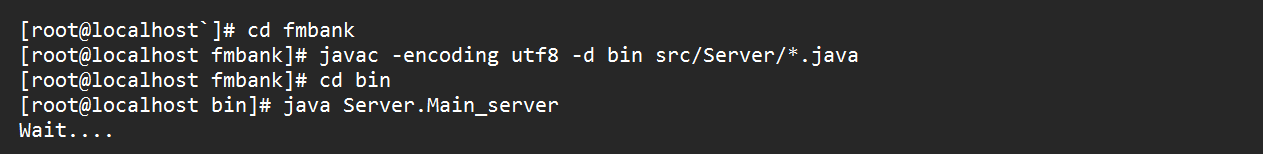
\includegraphics[width=0.8\textwidth]{figure/图1}
	\label{fig:example}
\end{figure}
3、启动客户端程序
首先进入项目文件fmbank,之后输入如下命令编译代码:
\\\\
\begin{adjustbox}{minipage=\linewidth, margin=0pt 0pt 2cm 0pt}
	\texttt{javac -encoding utf8 -d bin -cp .;lib\textbackslash jxl-2.6.12.jar;itextpdf-5.5.8.jar; src\textbackslash*Client\textbackslash*.java}
\end{adjustbox}
\\\\
其中-cp命令表示编译时引入第三方包。
之后进入bin文件,输入如下命令启动程序:
\\\\
\begin{adjustbox}{minipage=\linewidth, margin=0pt 0pt 2cm 0pt}
	\texttt{java -cp .;..\textbackslash lib\textbackslash jxl-2.6.12.jar;..\textbackslash lib\textbackslash itextpdf-5.5.8.jar; Client.Main\_client}
\end{adjustbox}
\\\\
出现如图界面表示启动成功:
\begin{figure}
	\centering
	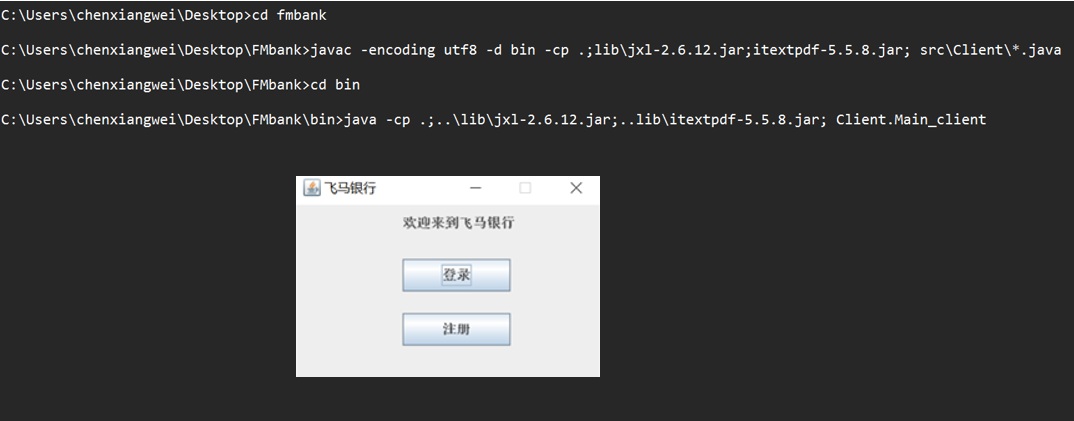
\includegraphics[width=0.8\textwidth]{figure/图2}
	\label{fig:example}
\end{figure}
\newpage
\section{结果展示}
1、注册功能\\
\begin{centering}
	\centering
	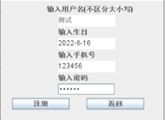
\includegraphics[width=0.8\textwidth]{figure/图3}
	\label{fig:example}
\end{centering}\\
\begin{centering}
	\centering
	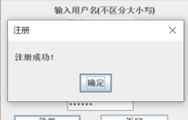
\includegraphics[width=0.8\textwidth]{figure/图4}
	\label{fig:example}
\end{centering}\\
2、登录功能\\
\begin{centering}
	\centering
	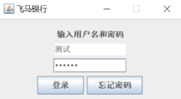
\includegraphics[width=0.8\textwidth]{figure/图5}
	\label{fig:example}
\end{centering}\\
\begin{centering}
	\centering
	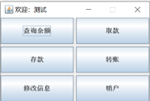
\includegraphics[width=0.8\textwidth]{figure/图6}
	\label{fig:example}
\end{centering}\\
3、查询功能\\
\begin{centering}
	\centering
	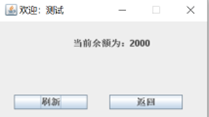
\includegraphics[width=0.8\textwidth]{figure/图7}
	\label{fig:example}
\end{centering}\\
4、存款功能\\
\begin{centering}
	\centering
	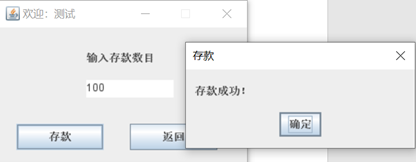
\includegraphics[width=0.8\textwidth]{figure/图8}
	\label{fig:example}
\end{centering}\\
\begin{centering}
	\centering
	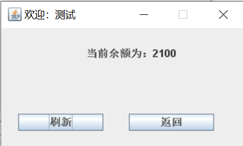
\includegraphics[width=0.8\textwidth]{figure/图9}
	\label{fig:example}
\end{centering}\\
5、取款功能\\
\begin{centering}
	\centering
	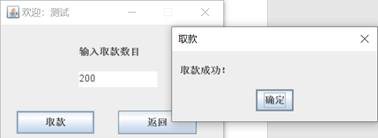
\includegraphics[width=0.8\textwidth]{figure/图10}
	\label{fig:example}
\end{centering}\\
\begin{centering}
	\centering
	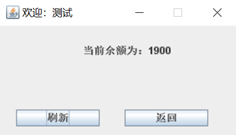
\includegraphics[width=0.8\textwidth]{figure/图11}
	\label{fig:example}
\end{centering}\\
6、转账功能\\
\begin{centering}
	\centering
	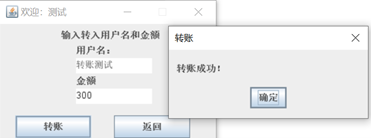
\includegraphics[width=0.8\textwidth]{figure/图12}
	\label{fig:example}
\end{centering}\\
\begin{centering}
	\centering
	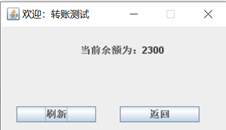
\includegraphics[width=0.8\textwidth]{figure/图13}
	\label{fig:example}
\end{centering}\\
7、销户功能\\
\begin{centering}
	\centering
	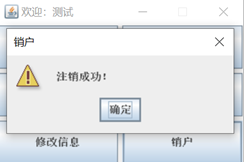
\includegraphics[width=0.8\textwidth]{figure/图14}
	\label{fig:example}
\end{centering}\\
8、报表功能\\
当用用户名root(管理员默认密码为八个八)登录时,会跳转到管理员界面,在管理员界面可以使用批量注册和生成报表功能。\\
\begin{centering}
	\centering
	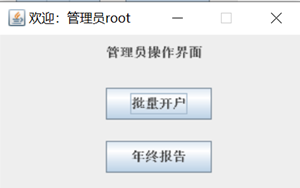
\includegraphics[width=0.8\textwidth]{figure/图15}
	\label{fig:example}
\end{centering}


\input{chapter/conclusion.tex}

\input{chapter/reference.tex}

\appendix

\newpage
\section{客户端Client部分代码}
\begin{lstlisting}[language = java, caption = Main\_Client.java]
package Client;

public class Main_client {
	public static void main(String[] args) {
		new UI("欢迎:",300,200);
	}
}
\end{lstlisting}
\begin{lstlisting}[language = java, caption = Client.java]
package Client;

import java.net.*;
import java.io.*;

public class Client {
	private String name;
	private int port;
	
	Client(String name, int port) {
		this.name = name;
		this.port = port;
	}
	
	/**
	* 执行客户端的工作,向服务器发送数据并接收响应
	* 
	* @param data 要发送给服务器的数据
	* @return 从服务器接收到的响应
	*/
	public String work(String data) {
		String res = "Null";
		try {
			// 创建与服务器的套接字连接,使用指定的名称和端口号
			Socket c = new Socket(name, port);
			
			// 获取套接字的输出流,并使用DataOutputStream进行包装以便写入数据
			OutputStream outToServer = c.getOutputStream();
			DataOutputStream out = new DataOutputStream(outToServer);
			
			// 将数据写入服务器
			out.writeUTF(data);
			
			// 获取套接字的输入流,并使用DataInputStream进行包装以便读取数据
			InputStream inFromServer = c.getInputStream();
			DataInputStream in = new DataInputStream(inFromServer);
			
			// 从服务器读取响应
			res = in.readUTF();
			
			// 关闭套接字连接
			c.close();
		} catch (SocketException se) {
			// 处理可能发生的套接字异常
			// (例如,如果连接被拒绝或服务器不可用)
		} catch (IOException e) {
			// 处理可能发生的其他输入/输出异常
		}
		// 返回从服务器接收到的响应
		return res;
	}
}
\end{lstlisting}
\begin{lstlisting}[language = java, caption = UI.java]
UI.java
package Client;

import java.awt.*;
import javax.swing.*;
import java.awt.event.ActionEvent;
import java.awt.event.ActionListener;

public class UI implements ActionListener{   
	
	// 用户参数
	private Worker w;
	private String usr;
	private String pas;
	private int count;
	
	// 参数
	private String Title;
	private int size1;
	private int size2;
	private final int xloc = 400;
	private final int yloc = 300;
	
	private JFrame current;
	private JFrame frame1;
	private JFrame frame2;
	private JFrame frame3;
	private JFrame frame4;
	private JFrame frame5;
	private JFrame frame6;
	private JFrame frame7;
	private JFrame frame8;
	private JFrame frame9;
	private JFrame frame10;
	
	// 回退
	private JButton bak1;
	private JButton bak2;
	private JButton bak3;
	private JButton bak4;
	private JButton bak5;
	private JButton bak6;
	// frame1
	private JButton btn1;
	private JButton btn2;
	// frame2
	private JButton btn3;
	private JButton btn4;
	// frame3
	private JButton btn5;
	private JButton btn6;
	private JButton btn7;
	private JButton btn8;
	private JButton btn9;
	private JButton btn10;
	// 查询余额
	private JButton btn15;
	//取款
	private JButton btn11;
	// 存款
	private JButton btn12;
	// 转账
	private JButton btn13;
	// 修改信息
	private JButton btn14;
	// 提交注册
	private JButton btn16;
	// 管理员操作
	private JButton btn17;
	private JButton btn18;
	
	// 卡片布局
	private CardLayout c1;
	private JPanel cards1;
	
	// 表单
	private JTextArea jta1;
	private JTextArea jta2;
	private JTextArea jta3;
	private JTextArea jta4;
	private JTextArea jta5;
	private JTextArea jta6;
	private JTextArea jta7;
	private JTextArea jta8;
	// 用户名
	private JTextArea jta9;
	// 生日
	private JTextArea jta10;
	// 手机号
	private JTextArea jta11;
	
	// 密码框
	private JPasswordField jpd1;
	private JPasswordField jpd2;
	private JPasswordField jpd3;
	// ...
	
	// 初始化
	UI(String title, int size1, int size2) {
		this.w = new Worker();
		this.Title = title;
		this.size1 = size1;
		this.size2 = size2;
		Frame1();
	}
	
	// 初始界面
	private void Frame1() {
		frame1 = new JFrame("飞马银行");
		frame1.setBounds(xloc,yloc,size1,size2);
		frame1.setResizable(false);
		frame1.setDefaultCloseOperation(JFrame.EXIT_ON_CLOSE);
		frame1.setLayout(null);
		frame1.setBackground(Color.gray);
		
		JLabel label = new JLabel("欢迎来到飞马银行");
		
		btn1 = new JButton("登录");
		btn2 = new JButton("注册");
		
		label.setBounds(100,2,200,30);
		btn1.setBounds(100,50,100,30);
		btn2.setBounds(100,100,100,30);
		
		btn1.addActionListener(this);
		btn2.addActionListener(this);
		
		frame1.add(label);
		frame1.add(btn1);
		frame1.add(btn2);
		
		current = frame1;
		current.setVisible(true);
	}
	
	// 登录界面
	private void Frame2() {
		frame2 = new JFrame("飞马银行");
		frame2.setBounds(xloc,yloc,size1,size2);
		frame2.setResizable(false);
		frame2.setDefaultCloseOperation(JFrame.EXIT_ON_CLOSE);
		frame2.setBackground(Color.gray);
		
		JPanel p = new JPanel();
		cards1 = new JPanel(new CardLayout(50,10));
		c1 = (CardLayout)(cards1.getLayout());
		
		JLabel label = new JLabel("输入用户名和密码");
		jta1 = new JTextArea(1,10);
		jpd1 = new JPasswordField(10);
		btn3 = new JButton("  登录  ");
		btn4 = new JButton("忘记密码");
		
		p.add(label);
		p.add(jta1);
		p.add(jpd1);
		p.add(btn3);
		p.add(btn4);
		
		cards1.add(p,"ok");
		frame2.add(cards1);
		
		btn3.addActionListener(this);
		btn4.addActionListener(this);
		
	}
	
	// 用户界面
	private void Frame3() {
		frame3 = new JFrame(Title+usr);
		frame3.setBounds(xloc,yloc,size1,size2);
		frame3.setResizable(false);
		frame3.setDefaultCloseOperation(JFrame.EXIT_ON_CLOSE);
		frame3.setBackground(Color.gray);
		
		btn5 = new JButton("查询余额");
		btn6 = new JButton("取款");
		btn7 = new JButton("存款");
		btn8 = new JButton("转账");
		btn9 = new JButton("修改信息");
		btn10 = new JButton("销户");
		
		frame3.add(btn5);
		frame3.add(btn6);
		frame3.add(btn7);
		frame3.add(btn8);
		frame3.add(btn9);
		frame3.add(btn10);
		
		frame3.setLayout(new GridLayout(3,2,5,5));
		
		btn5.addActionListener(this);
		btn6.addActionListener(this);
		btn7.addActionListener(this);
		btn8.addActionListener(this);
		btn9.addActionListener(this);
		btn10.addActionListener(this);
		
	}
	
	// 查询余额界面
	private void Frame4() {
		frame4 = new JFrame(Title+usr);
		//frame4.setSize(size1,size2);
		frame4.setBounds(xloc,yloc,size1,size2);
		frame4.setResizable(false);
		frame4.setDefaultCloseOperation(JFrame.EXIT_ON_CLOSE);
		frame4.setBackground(Color.gray);
		
		frame4.setLayout(null);
		
		JLabel label = new JLabel("当前余额为:"+count+"");
		btn15 = new JButton("刷新");
		bak1 = new JButton("返回");
		
		label.setBounds(100,20,150,20);
		btn15.setBounds(20,100,100,20);
		bak1.setBounds(150,100,100,20);
		
		frame4.add(label);
		frame4.add(btn15);
		frame4.add(bak1);
		
		btn15.addActionListener(this);
		bak1.addActionListener(this);
	}
	
	// 取款界面
	private void Frame5() {
		frame5 = new JFrame(Title+usr);
		frame5.setBounds(xloc,yloc,size1,size2);
		frame5.setResizable(false);
		frame5.setDefaultCloseOperation(JFrame.EXIT_ON_CLOSE);
		frame5.setBackground(Color.gray);
		frame5.setLayout(null);
		
		JLabel label = new JLabel("输入取款数目");
		jta2 = new JTextArea(1,10);
		btn11 = new JButton("取款");
		bak2 = new JButton("返回");
		
		label.setBounds(100,10,100,50);
		jta2.setBounds(100,60,100,20);
		btn11.setBounds(20,110,100,30);
		bak2.setBounds(150,110,100,30);
		
		frame5.add(label);
		frame5.add(jta2);
		frame5.add(btn11);
		frame5.add(bak2);
		
		
		btn11.addActionListener(this);
		bak2.addActionListener(this);
	}
	
	// 存款界面
	private void Frame6() {
		frame6 = new JFrame(Title+usr);
		frame6.setBounds(xloc,yloc,size1,size2);
		frame6.setResizable(false);
		frame6.setDefaultCloseOperation(JFrame.EXIT_ON_CLOSE);
		frame6.setBackground(Color.gray);
		
		frame6.setLayout(null);
		
		JLabel label = new JLabel("输入存款数目");
		jta3 = new JTextArea(1,10);
		btn12 = new JButton("存款");
		bak3 = new JButton("返回");
		
		btn12.addActionListener(this);
		bak3.addActionListener(this);
		
		label.setBounds(100,10,100,50);
		jta3.setBounds(100,60,100,20);
		btn12.setBounds(20,110,100,30);
		bak3.setBounds(150,110,100,30);
		
		frame6.add(label);
		frame6.add(jta3);
		frame6.add(btn12);
		frame6.add(bak3);
	}
	
	// 转账界面
	private void Frame7() {
		frame7 = new JFrame(Title+usr);
		frame7.setBounds(xloc,yloc,size1,size2);
		frame7.setResizable(false);
		frame7.setDefaultCloseOperation(JFrame.EXIT_ON_CLOSE);
		frame7.setBackground(Color.gray);
		
		frame7.setLayout(null);
		
		JLabel label1 = new JLabel("输入转入用户名和金额");
		JLabel label2 = new JLabel("用户名:");
		JLabel label3 = new JLabel("金额");
		jta4 = new JTextArea(1,10);
		jta5 = new JTextArea(1,10);
		btn13 = new JButton("转账");
		bak4 = new JButton("返回");
		
		btn13.addActionListener(this);
		bak4.addActionListener(this);
		
		label1.setBounds(80,5,150,20);
		label2.setBounds(100,25,100,20);
		jta4.setBounds(100,45,100,20);
		label3.setBounds(100,65,100,20);
		jta5.setBounds(100,85,100,20);
		btn13.setBounds(20,120,100,30);
		bak4.setBounds(150,120,100,30);
		
		frame7.add(label1);
		frame7.add(label2);
		frame7.add(jta4);
		frame7.add(label3);
		frame7.add(jta5);
		frame7.add(btn13);
		frame7.add(bak4);
	}
	
	// 修改信息界面
	private void Frame8() {
		frame8 = new JFrame(Title+usr);
		frame8.setBounds(xloc,yloc,size1,size2);
		frame8.setResizable(false);
		frame8.setDefaultCloseOperation(JFrame.EXIT_ON_CLOSE);
		frame8.setBackground(Color.gray);
		
		frame8.setLayout(null);
		
		JLabel label1 = new JLabel("新密码:");
		JLabel label2 = new JLabel("修改生日");
		JLabel label3 = new JLabel("修改手机号");
		jpd2 = new JPasswordField();
		jta7 = new JTextArea(1,10);
		jta8 = new JTextArea(1,10);
		btn14 = new JButton("修改");
		bak5 = new JButton("返回");
		
		btn14.addActionListener(this);
		bak5.addActionListener(this);
		
		label1.setBounds(100,5,100,20);
		jpd2.setBounds(100,25,100,20);
		label2.setBounds(100,45,100,20);
		jta7.setBounds(100,65,100,20);
		label3.setBounds(100,85,100,20);
		jta8.setBounds(100,105,100,20);
		btn14.setBounds(20,140,100,20);
		bak5.setBounds(150,140,100,20);
		
		frame8.add(label1);
		frame8.add(label2);
		frame8.add(label3);
		frame8.add(jpd2);
		frame8.add(jta7);
		frame8.add(jta8);
		frame8.add(btn14);
		frame8.add(bak5);
	}
	
	// 注册界面
	private void Frame9() {
		frame9 = new JFrame(Title);
		frame9.setBounds(xloc,yloc,size1,size2+50);
		frame9.setResizable(false);
		frame9.setDefaultCloseOperation(JFrame.EXIT_ON_CLOSE);
		frame9.setBackground(Color.gray);
		
		frame9.setLayout(null);
		
		JLabel label1 = new JLabel("输入用户名(不区分大小写)");
		JLabel label2 = new JLabel("输入生日");
		JLabel label3 = new JLabel("输入手机号");
		JLabel label4 = new JLabel("输入密码");
		jta9 = new JTextArea(1,10);
		jta10 = new JTextArea(1,10);
		jta11 = new JTextArea(1,10);
		jpd3 = new JPasswordField();
		btn16 = new JButton("注册");
		bak6 = new JButton("返回");
		
		label1.setBounds(80,5,200,20);
		jta9.setBounds(100,25,100,20);
		label2.setBounds(100,45,100,20);
		jta10.setBounds(100,65,100,20);
		label3.setBounds(100,85,100,20);
		jta11.setBounds(100,105,100,20);
		label4.setBounds(100,125,100,20);
		jpd3.setBounds(100,145,100,20);
		btn16.setBounds(20,170,100,20);
		bak6.setBounds(150,170,100,20);
		
		btn16.addActionListener(this);
		bak6.addActionListener(this);
		
		frame9.add(label1);
		frame9.add(label2);
		frame9.add(label3);
		frame9.add(label4);
		frame9.add(jta9);
		frame9.add(jta10);
		frame9.add(jta11);
		frame9.add(jpd3);
		frame9.add(btn16);
		frame9.add(bak6);
	}
	
	// 管理员界面
	private void Frame10() {
		frame10 = new JFrame(Title+"管理员"+usr);
		frame10.setBounds(xloc,yloc,size1,size2);
		frame10.setResizable(false);
		frame10.setDefaultCloseOperation(JFrame.EXIT_ON_CLOSE);
		frame10.setLayout(null);
		frame10.setBackground(Color.gray);
		
		JLabel label = new JLabel("管理员操作界面");
		
		btn17 = new JButton("批量开户");
		btn18 = new JButton("年终报告");
		
		label.setBounds(100,2,200,30);
		btn17.setBounds(100,50,100,30);
		btn18.setBounds(100,100,100,30);
		
		btn17.addActionListener(this);
		btn18.addActionListener(this);
		
		frame10.add(label);
		frame10.add(btn17);
		frame10.add(btn18);
		
	}
	
	// ...
	
	
	
	// 事件监听
	public void actionPerformed(ActionEvent e) {
		if(e.getSource() == bak6) bak0();
		else if(e.getSource() == bak1 || e.getSource() == bak2 || e.getSource() == bak3 || e.getSource() == bak4 || e.getSource() == bak5) bak();
		else if(e.getSource() == btn1) btn_1();
		else if(e.getSource() == btn2) btn_2();
		else if(e.getSource() == btn3) btn_3();
		else if(e.getSource() == btn4) btn_4();
		else if(e.getSource() == btn5) btn_5();
		else if(e.getSource() == btn6) btn_6();
		else if(e.getSource() == btn7) btn_7();
		else if(e.getSource() == btn8) btn_8();
		else if(e.getSource() == btn9) btn_9();
		else if(e.getSource() == btn10) btn_10();
		else if(e.getSource() == btn11) btn_11();
		else if(e.getSource() == btn12) btn_12();
		else if(e.getSource() == btn13) btn_13();
		else if(e.getSource() == btn14) btn_14();
		else if(e.getSource() == btn15) btn_15();
		else if(e.getSource() == btn16) btn_16();
		else if(e.getSource() == btn17) btn_17();
		else if(e.getSource() == btn18) btn_18();
	}
	
	// 返回按钮
	private void bak() {
		current.setVisible(false);
		frame3.setVisible(true);
		current = frame3;
	}
	
	private void bak0() {
		current.setVisible(false);
		frame1.setVisible(true);
		current = frame1;
	}
	
	
	// 跳转登录界面
	private void btn_1() {
		Frame2();
		current.setVisible(false);
		frame2.setVisible(true);
		c1.show(cards1,"ok");
		current = frame2;
	}
	
	// 跳转创建账户页面
	private void btn_2() {
		Frame9();
		current.setVisible(false);
		frame9.setVisible(true);
		current = frame9;
	}
	
	// 跳转用户页面
	private void btn_3() {
		usr = jta1.getText();
		pas = new String(jpd1.getPassword());
		if(w.check_login(usr,pas) == false) {
			JOptionPane.showMessageDialog(frame2, "密码或用户名错误!","错误",2);
		} else {
			if(usr.equals("root")) {
				Frame10();
				current.setVisible(false);
				frame10.setVisible(true);
				current = frame10;
			} else {
				Frame3();
				current.setVisible(false);
				frame3.setVisible(true);
				current = frame3;
			}
		}
	}
	
	// 忘记密码
	private void btn_4() {
		JOptionPane.showMessageDialog(frame2, "仔细回忆","忘记密码",1);
	}
	
	// 跳转查询余额页面
	private void btn_5() {
		Frame4();
		count = w.check_money(usr);
		Frame4();
		current.setVisible(false);
		frame4.setVisible(true);
		current = frame4;
	}
	
	// 跳转取款页面
	private void btn_6() {
		Frame5();
		current.setVisible(false);
		frame5.setVisible(true);
		current = frame5;
	}
	
	// 跳转存款页面
	private void btn_7() {
		Frame6();
		current.setVisible(false);
		frame6.setVisible(true);
		current = frame6;
	}
	
	// 跳转转账页面
	private void btn_8() {
		Frame7();
		current.setVisible(false);
		frame7.setVisible(true);
		current = frame7;
	}
	
	// 跳转修改信息页面
	private void btn_9() {
		Frame8();
		current.setVisible(false);
		frame8.setVisible(true);
		current = frame8;
	}
	
	// 销户
	private void btn_10() {
		if(w.logout(usr)) {
			JOptionPane.showMessageDialog(frame3, "注销成功!","销户",2);
			btn_1();
		}
	}
	
	// 取款提交
	private void btn_11() {
		try {
			int withdraw = Integer.parseInt(jta2.getText());
			// System.out.println(withdraw);
			w.withdraw_money(usr, withdraw);
			JOptionPane.showMessageDialog(frame5, "取款成功!","取款",JOptionPane.PLAIN_MESSAGE);
		} catch (Exception e) {JOptionPane.showMessageDialog(frame5, "请输入数字!","格式错误",2);}
		
	}
	
	// 存款提交
	private void btn_12() {
		try {
			int store = Integer.parseInt(jta3.getText());
			// System.out.println(store);
			w.store_money(usr, store);
			JOptionPane.showMessageDialog(frame6, "存款成功!","存款",JOptionPane.PLAIN_MESSAGE);
		} catch (Exception e) {JOptionPane.showMessageDialog(frame6, "请输入数字!","格式错误",2);}
	}
	
	// 转账提交
	private void btn_13() {
		try {
			String tousr = jta4.getText();
			int transfer = Integer.parseInt(jta5.getText());
			if(tousr.equals("root")) {
				JOptionPane.showMessageDialog(frame7, "禁止向管理员转账!","错误",2);
			} else {
				if(w.transfer(usr, tousr, transfer) == false) JOptionPane.showMessageDialog(frame7, "转账失败!用户不存在或余额不足!","转账",JOptionPane.PLAIN_MESSAGE);
				else JOptionPane.showMessageDialog(frame7, "转账成功!","转账",JOptionPane.PLAIN_MESSAGE);
			}
		} catch (Exception e) {JOptionPane.showMessageDialog(frame7, "请输入数字!","格式错误",2);}
		
	}
	
	// 修改信息提交
	private void btn_14() {
		String pas = new String(jpd2.getPassword());
		String birth = jta7.getText();
		String phone = jta8.getText();
		if(w.update_info(usr, pas, birth, phone)) {
			JOptionPane.showMessageDialog(frame8, "修改成功!","修改",JOptionPane.PLAIN_MESSAGE);
		}
	}
	
	// 余额刷新
	private void btn_15() {
		btn_5();
	}
	
	// 注册提交
	private void btn_16() {
		String usr_name = jta9.getText();
		String birth = jta10.getText();
		String phone = jta11.getText();
		String pass = new String(jpd3.getPassword());
		if(w.signin(usr_name, birth, phone, pass, 1, 9941, 2000) == false) {
			JOptionPane.showMessageDialog(frame9, "用户名重复!","注册失败",2);
		} else {
			JOptionPane.showMessageDialog(frame9, "注册成功!","注册",JOptionPane.PLAIN_MESSAGE);
			btn_1();
		}
	}
	
	// 批量开户
	private void btn_17() {
		JFileChooser fc = new JFileChooser("C:\\");
		int val = fc.showOpenDialog(frame10);
		if(val == fc.APPROVE_OPTION) {
			System.out.println(fc.getSelectedFile().toString());
			int res = w.bulk_signin(fc.getSelectedFile().toString());
			if(res == -1) {
				JOptionPane.showMessageDialog(frame10, "文件格式错误或不支持xlsx格式,请使用xls格式!","文件格式错误",2);
			} else {
				JOptionPane.showMessageDialog(frame10, "成功注册"+res+"个用户!","成功",JOptionPane.PLAIN_MESSAGE);
			}
		}
	}
	
	// 年终报告
	private void btn_18() {
		if(w.createpdf(".\\REPORT.pdf")) {
			JOptionPane.showMessageDialog(frame10, "生成报告成功!文件在当前目录中。","生成报告",JOptionPane.PLAIN_MESSAGE);
		} else {
			JOptionPane.showMessageDialog(frame10, "生成报告失败!","生成报告",2);
		}
	}
	
}
\end{lstlisting}
\begin{lstlisting}[language = java, caption = Worker.java]
package Client;

import java.io.File;
import java.io.FileOutputStream;
import java.io.IOException;
import jxl.*;
import jxl.read.biff.BiffException;
import com.itextpdf.text.Document;
import com.itextpdf.text.DocumentException;
import com.itextpdf.text.Paragraph;
import com.itextpdf.text.pdf.PdfWriter;


public class Worker {
	private Client c;
	
	// 格式:flag(有返回值为0) + number(int为1) + length(column) + column + sql
	// 表: id(int2), usr(string3), pass(string4), schn(int4), phone(string5), sex(int3), birth(string5), money(int5)
	
	// 构造,初始化
	Worker() {
		this.c = new Client("192.168.66.128",6606);
	}
	
	// 查询用户是否存在 不存在返回true,存在返回false
	private boolean check_usr(String usr) {
		return send_msg("012idSELECT id FROM fmbank WHERE usr='"+usr+"';").equals("Null");
	}
	
	// 判断是否登录成功
	public boolean check_login(String usr, String pass) {
		if(check_usr(usr) == true) return false;
		return send_msg("004passSELECT pass FROM fmbank WHERE usr='"+usr+"';").equals(pass);
	}
	
	// 发送数据
	private String send_msg(String data) {
		return c.work(data);
	}
	
	// 余额查询,返回余额
	public int check_money(String usr) {
		return Integer.parseInt(send_msg("015moneySELECT money FROM fmbank WHERE usr='"+usr+"';"));
	}
	
	// 取款,返回是否成功
	public boolean withdraw_money(String usr, int money) {
		int count = check_money(usr);
		if(count < money) return false;
		count -= money;
		send_msg("1UPDATE fmbank SET money="+count+" WHERE usr='"+usr+"';");
		return true;
	}
	
	// 存款,返回是否存款成功
	public boolean store_money(String usr, int money) {
		int count = check_money(usr);
		count += money;
		send_msg("1UPDATE fmbank SET money="+count+" WHERE usr='"+usr+"';");
		return true;
	}
	
	// 转账,返回是否转账成功
	public boolean transfer(String fromusr, String tousr, int money) {
		if(check_usr(tousr) == true) return false;
		boolean res = withdraw_money(fromusr,money);
		if(res == false) return res;
		return store_money(tousr,money);
	}
	
	// 注册,返回是否注册成功
	public boolean signin(String usr_name, String birth, String phone, String pass, int sex, int schn, int money) {
		if(check_usr(usr_name) == false) return false;
		send_msg("1INSERT INTO fmbank (usr,pass,schn,phone,sex,birth,money) VALUES ('"+usr_name+"','"+pass+"',"+schn+",'"+phone+"',"+sex+",'"+birth+"',"+money+");");
		return true;
	}
	
	// 批量注册, 返回是否成功
	public int bulk_signin(String file_name) {
		int cnt = 0;
		try {
			Workbook book = Workbook.getWorkbook(new File(file_name));
			Sheet sheet = book.getSheet(0);
			int cols = sheet.getColumns();
			int rows = sheet.getRows();
			for(int i = 0; i < rows; i++) {
				String usr,birth,phone,pass,sex,schn;
				usr = birth = phone = pass = sex = schn = null;
				for(int j = 0; j < cols; j++) {
					switch(j) {
						case 0: usr = sheet.getCell(j, i).getContents(); break;
						case 1: birth = sheet.getCell(j, i).getContents(); break;
						case 2: phone = sheet.getCell(j, i).getContents(); break;
						case 3: pass = sheet.getCell(j, i).getContents(); break;
						case 4: sex = sheet.getCell(j, i).getContents(); break;
						case 5: schn = sheet.getCell(j, i).getContents(); break;
					}
				}
				int sex_, schn_;
				try {
					sex_ = Integer.parseInt(sex);
				} catch (NumberFormatException e) {sex_ = -1;}
				try {
					schn_ = Integer.parseInt(schn);
				} catch (NumberFormatException e) {schn_ = -1;}
				signin(usr,birth,phone,pass,sex_,schn_,2000);
				cnt++;
			}
		} catch (IOException e) {
			return -1;
		} catch (BiffException e) {
			return -1;
		}
		return cnt;
	}
	
	// 注销用户,返回是否注销成功
	public boolean logout(String usr) {
		send_msg("1DELETE FROM fmbank WHERE usr='"+usr+"';");
		return true;
	}
	
	// 修改信息, 返回是否修改成功
	public boolean update_info(String usr, String pass, String birth, String phone) {
		send_msg("1UPDATE fmbank SET pass='"+pass+"',birth='"+birth+"',phone='"+phone+"' WHERE usr='"+usr+"';");
		return true;
	}
	
	// 年终报告
	public boolean createpdf(String file_name) {
		try {
			Document document = new Document();
			PdfWriter.getInstance(document, new FileOutputStream(file_name));
			int account = Integer.parseInt(send_msg("014numsSELECT COUNT(*) AS nums FROM fmbank;"));
			int count = Integer.parseInt(send_msg("014numsSELECT SUM(money) AS nums FROM fmbank;"));
			document.open();
			document.add(new Paragraph("Fei Ma Bank annual report"));
			document.add(new Paragraph("The total number of the account is: "+account));
			document.add(new Paragraph("The number of the new account is: "+account));
			document.add(new Paragraph("The total cash in the bank are: "+count));
			document.close();
			return true;
		} catch (DocumentException e) {
			return false;
		} catch (IOException e) {
			return false;
		}
	}
}
\end{lstlisting}
\newpage
\section{服务器端Server部分的代码}
\begin{lstlisting}[language = java, caption = Main\_Server.java]
package Server;

import java.net.*;
import java.io.*;

public class Main_server {
	public static void main(String[] args) {
		ServerSocket socket = null;
		Socket s = null;
		try {
			// 创建服务器Socket,监听指定端口
			socket = new ServerSocket(6606);
		} catch (IOException e) {
			e.printStackTrace();
		}
		System.out.println("等待连接....");
		while (true) {
			try {
				// 等待客户端连接
				s = socket.accept();
				// 创建新的线程处理客户端请求
				new Thread(new Server(s)).start();
			} catch (IOException e) {
				e.printStackTrace();
			}
		}
	}
}
\end{lstlisting}
\begin{lstlisting}[language = java, caption = Server.java]
package Server;

import java.net.*;
import java.io.*;

public class Server implements Runnable {
	private Operator opr;
	private DB data_base;
	private Socket s;
	
	Server(Socket s) {
		this.s = s;
		this.data_base = new DB();
		this.opr = new Operator();
	}
	
	// 线程执行的主体方法
	public void run() {
		System.out.println("远程主机连接,地址为:" + this.s.getRemoteSocketAddress());
		try {
			DataInputStream in = new DataInputStream(this.s.getInputStream());
			String rec = in.readUTF();
			System.out.println("接收命令:" + rec);
			DataOutputStream out = new DataOutputStream(this.s.getOutputStream());
			if (opr.get_flag(rec).equals("1")) {
				// 执行数据库更新操作
				data_base.db_exe(opr.get_sql(rec));
				out.writeUTF("done");
			} else {
				// 执行数据库查询操作
				out.writeUTF(data_base.db_query(opr.get_sql(rec), opr.get_col(rec), opr.get_f(rec)));
			}
		} catch (IOException e) {
			// 处理异常
		}
	}
	
	public static void main(String[] args) {
		// 主函数,用于启动服务器
	}
}
\end{lstlisting}
\begin{lstlisting}[language = java, caption = DB.java]
package Server;

import java.sql.*;

public class DB {
	static final String JDBC_DRIVER = "com.mysql.cj.jdbc.Driver";  
	static final String DB_URL = "jdbc:mysql://localhost/testgb";
	
	static final String USER = "root";
	static final String PASS = "2%duLg7dWiND";
	
	private Connection conn;
	private Statement stmt;
	
	// 构造函数,初始化数据库连接
	DB() {
		try {
			Class.forName(JDBC_DRIVER);
			
			System.out.println("连接到数据库...");
			conn = DriverManager.getConnection(DB_URL, USER, PASS);
			stmt = conn.createStatement();
		} catch (SQLException se) {
			se.printStackTrace();
		} catch (Exception e) {
			e.printStackTrace();
		}
		System.out.println("连接成功。");
	}
	
	// 执行数据库查询并返回结果
	public synchronized String db_query(String sql, String col, int flag) {
		String res = "Null";
		try {
			ResultSet rs = stmt.executeQuery(sql);
			if (flag == 1)
			while (rs.next())
			res = rs.getInt(col) + "";
			else
			while (rs.next())
			res = rs.getString(col);
		} catch (SQLException se) {
			se.printStackTrace();
		} catch (Exception e) {
			e.printStackTrace();
		}
		return res;
	}
	
	// 执行数据库操作
	public synchronized void db_exe(String sql) {
		try {
			stmt.execute(sql);
		} catch (SQLException se) {
			se.printStackTrace();
		} catch (Exception e) {
			e.printStackTrace();
		}
	}
}
\end{lstlisting}
\begin{lstlisting}[language = java, caption = Operator.java]
package Server;

public class Operator {
	// 114abcd sql
	// 格式:flag + number + length(column) + column + sql
	
	public String get_flag(String s) {
		// 获取命令标志位(flag)
		return s.charAt(0) + "";
	}
	
	public String get_col(String s) {
		if ((s.charAt(0) + "").equals("0")) {
			int st = Integer.parseInt(s.charAt(2) + "");
			// 获取列名(column)
			return s.substring(3, st + 3);
		} else {
			return "";
		}
	}
	
	public int get_f(String s) {
		if ((s.charAt(0) + "").equals("0")) {
			// 获取查询标志位(flag)
			return Integer.parseInt(s.charAt(1) + "");
		} else {
			return -1;
		}
	}
	
	public String get_sql(String s) {
		if ((s.charAt(0) + "").equals("0")) {
			int st = Integer.parseInt(s.charAt(2) + "");
			// 获取SQL语句
			return s.substring(st + 3);
		} else {
			return s.substring(1);
		}
	}
}
\end{lstlisting}

\end{document}